\section{Segmentation}

The first step is to take a given image or scene and extract the individual objects.

Typically this can be a complex problem to tackle as stafflines connect almost all components together and must therefore first be removed. Also some musical entities are themselves comprised of multiple other entities. Good examples are the bass clef which is comprised of two dots placed above each other to the right of the curve and dotted notes , both of which can be seen in \todo[inline]{Examples of multi-component musical entities}.

Particularly in this project, we also need to be able to break down the musical entities further into stems and note heads and so separating these from each other present another problem which we must take into account.

\subsection{Connected Component Analysis}

\subsection{Projections}

The technique essentially involves projecting the manuscript in the x and y axes, collecting the pixels in either individual pixel lines or buckets in order to help establish information about the image.

Mathematically, if the image is represented as a 1 bit (2 colour) image $I(x_{\text{max}}, y_{\text{max}})$ of width $x_{\text{max}}$ and height $y_{\text{max}}$, let $p_{xy} \in 0, 1$ denotes the value for a specific pixel at row $y$ column $x$.

The horizontal and vertical projections can then be defined as:


\begin{equation} \label{eq:hproj}
  \text{Proj}_{\text{horizontal}}(y) = \sum_{j = 0}^{x_\text{max}} p_{jy}
\end{equation}

\begin{equation} \label{eq:vproj}
  \text{Proj}_{\text{vertical}}(x) = \sum_{j = 0}^{y_\text{max}} p_{xj}
\end{equation}

\begin{figure}[h!]
  \centering
  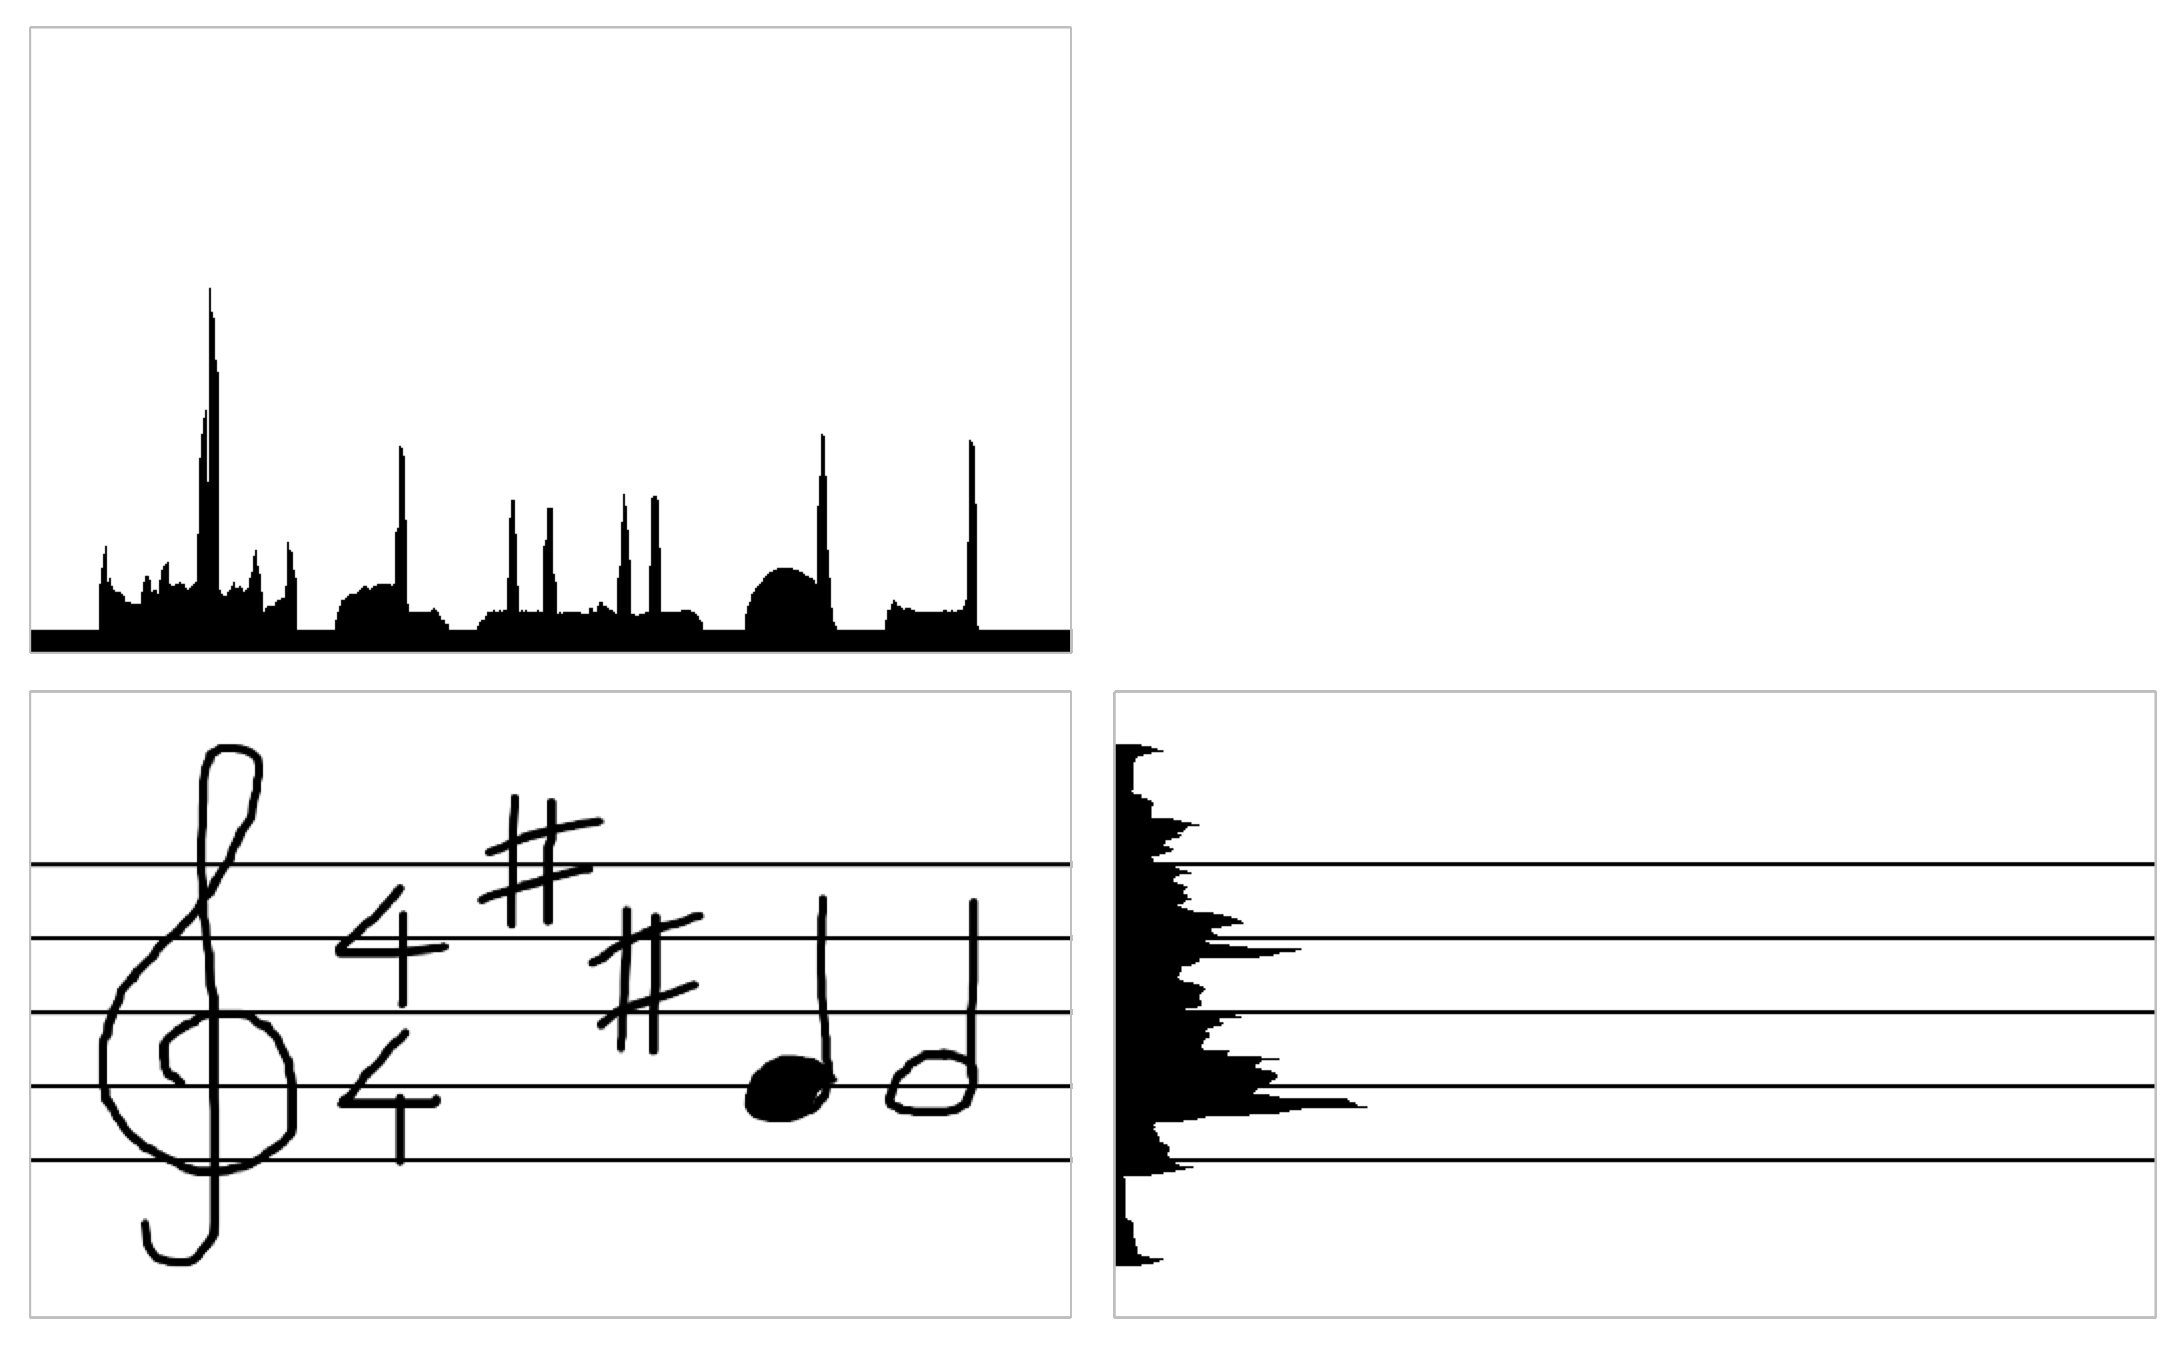
\includegraphics[width=\linewidth]{gfx/technical-background/projection.png}
  \caption{Horizontal and Vertical Projections of handwritten music excerpt}
  \label{fig:stave-projection}
\end{figure}

An example section of score is shown in figure \ref{fig:stave-projection} and you can immediately see the potential for use in detection/removal of staff lines using equation \eqref{eq:hproj} or in isolation and segmentation of components using equation \eqref{eq:vproj}.
